\chapter{Problem Definition and Task Specifications}
\label{chapter:problem}

This chapter provides a formal definition of the Multi-Turn Retrieval-Augmented Generation (RAG) problem under sequential decision constraints. It delineates the structural specifications of the MTRAGEval benchmark (SemEval-2026 Task~8), conducts an empirical analysis of the underlying multi-domain corpora, profiles the evaluation metrics, and establishes the formal research questions and hypotheses that guide the experimental framework developed in Chapter~5 and evaluated in Chapter~6.

%==============================================================
\section{Formal Mathematical Formulation}
\label{sec:formal-formulation}
%==============================================================

We formalize multi-turn conversational RAG as a sequential process unfolding over a set of discrete dialogue turns indexed by $t \in \{1, 2, \dots, L\}$, where $L$ is the length of the conversation. At any given turn $t$, the state of the conversation is fully encapsulated by the user--agent history window, denoted $H_t$:
\begin{equation}
H_t = \Big( (u_1, \mathcal{D}_1, y_1), (u_2, \mathcal{D}_2, y_2), \dots, (u_{t-1}, \mathcal{D}_{t-1}, y_{t-1}) \Big)
\end{equation}
where $u_i$ is the raw user utterance at turn $i$, $\mathcal{D}_i$ is the subset of document passages retrieved at turn $i$, and $y_i$ is the agent response at turn $i$. In a deployed assistant, $\mathcal{D}_i$ and $y_i$ are the system's own earlier outputs; in the MTRAGEval benchmark used in this thesis, the history is the benchmark's \emph{reference} conversation, so earlier system errors do not enter $H_t$. At the current turn $t$, the user introduces a new conversational utterance $u_t$, which defines the active query $q_t \equiv u_t$. The system has access to a massive, static global corpus $\mathcal{D} = \{d_1, d_2, \dots, d_{|\mathcal{D}|}\}$.

The objective of multi-turn RAG decomposes into three separate probabilistic functions, evaluated explicitly under the tripartite MTRAGEval specification. These three functions are not merely three ways of measuring the same underlying capability---each isolates a distinct point of potential failure in the pipeline, which is precisely why the MTRAGEval competition (and this thesis) evaluates them independently rather than only end-to-end.

Table~\ref{tab:notation} summarizes the principal notation used throughout the thesis.

\begin{table}[h]
\centering
\small
\begin{tabular}{ll}
\toprule
\textbf{Symbol} & \textbf{Meaning} \\
\midrule
$t$, $L$ & Turn index; number of turns in a conversation \\
$u_t$, $q_t$ & User utterance at turn $t$; active query ($q_t \equiv u_t$) \\
$H_t$ & Conversation history available at turn $t$ \\
$\mathcal{D}$, $\mathcal{D}_t$, $\mathcal{D}_t^*$ & Corpus; passages retrieved at turn $t$; gold reference passages \\
$\mathcal{S}_t$ & Verbatim evidence spans extracted at turn $t$ \\
$y_t$, $y_t^*$ & Generated response; reference response \\
$z_t$, $\hat{z}_t$ & True answerability label; answerability decision of the gate \\
$\tau$ & Confidence threshold of the answerability gate ($\tau{=}0.7$) \\
$T$ & LLM sampling temperature (and temperature of the contrastive loss in Section~\ref{sec:ir-paradigms}) \\
$k$ & Rank-decay constant of (weighted) RRF ($k_{\text{internal}}$, $k_{\text{final}}^{(c)}$ in Nested RRF) \\
$\alpha$ & Weight of the reranker signal in the hybrid fusion \\
$w_s^{(c)}$ & Nested RRF weight of input $s$ for corpus $c$ \\
$N$, $K$ & Passages retrieved per reformulation; maximum number of extracted spans \\
$r_4$, $\phi(r_4)$ & 4-gram overlap with the evidence spans; extractiveness shaping function \\
\bottomrule
\end{tabular}
\caption{Principal notation.}
\label{tab:notation}
\end{table}

\subsection{Task A: Multi-Turn Passage Retrieval Specification}

The objective of Task~A is to evaluate conversational search \textit{independently of downstream generation}, isolating retrieval quality from any confound introduced by the generator. Given the conversational history $H_t$ and the active, potentially non-standalone query $q_t$, the retrieval module $\mathcal{R}$ must produce a ranked list $\mathcal{D}_t$ containing exactly the top-$k$ (with $k{=}10$ under the competition specification) most relevant passages extracted from the global corpus $\mathcal{D}$, sorted by decreasing order of semantic relevance to $q_t$ under the context of $H_t$:
\begin{equation}
\mathcal{R}(q_t, H_t, \mathcal{D}) \;\longrightarrow\; \mathcal{D}_t = \big\{d_{(1)}, d_{(2)}, \dots, d_{(k)}\big\}, \quad d_{(i)} \in \mathcal{D}, \quad k=10
\end{equation}

\subsection{Task B: Reference-Grounded Response Generation Specification}

The objective of Task~B is to isolate \textit{generation} quality from retrieval mechanics by entirely removing the search bottleneck. The system is provided with the true dialogue history $H_t$, the active query $q_t$, and a fixed set of gold-standard relevant reference passages $\mathcal{D}_t^* \subset \mathcal{D}$. The generator function $\mathcal{G}$ must synthesize a natural-language response $y_t$ that is strictly grounded in $\mathcal{D}_t^*$, maximizing factual alignment while avoiding out-of-context abstraction:
\begin{equation}
\mathcal{G}(q_t, H_t, \mathcal{D}_t^*) \;\longrightarrow\; y_t
\end{equation}

\subsection{Task C: End-to-End Retrieval-Augmented Generation Specification}

Task~C unifies retrieval and generation, mirroring real-world deployment conditions in which no gold evidence set is ever supplied at inference time. Given only $H_t$, $q_t$, and the raw global corpus $\mathcal{D}$, the architecture must first retrieve up to $10$ relevant passages using its own internal retrieval module, and subsequently condition its generator on these \textit{noisy, self-retrieved} documents to produce the final response $y_t$. Because the retrieved set $\mathcal{D}_t$ is no longer guaranteed to be relevant, Task~C requires the system to additionally model a latent binary answerability variable $z_t \in \{0,1\}$:
\begin{equation}
z_t =
\begin{cases}
1, & \text{if } \mathcal{D}_t \text{ contains sufficient evidence to fully justify an answer to } q_t \\
0, & \text{otherwise (unanswerable turn)}
\end{cases}
\end{equation}
The end-to-end objective therefore reduces to mapping $[q_t, H_t, \mathcal{D}]$ to an output pair $(\mathcal{D}_t, y_t)$, maximizing factual grounding if $\hat{z}_t = 1$, or executing a calibrated refusal if $\hat{z}_t = 0$. As we show in Chapter~6, this additional decision layer---absent from Tasks A and B by construction---is a major source of the additional difficulty of Task~C, together with the fact that generation must rely on system-retrieved rather than reference passages.

\subsection{A Unified Optimization Perspective}
\label{sec:unified-objective}

Tasks A, B, and C are not merely three independent evaluation protocols; they are three coordinates of a single underlying design objective. It is useful, before turning to the concrete system of Chapter~5, to state this objective explicitly in idealized form, even though---as discussed below---it is not the objective actually optimized by the system. Let $\mathcal{X}$ denote the distribution of (query, history) pairs induced by the benchmark, and let $y_t^*$, $\mathcal{D}_t^*$ denote the human reference response and gold evidence set for turn $t$. The architecture as a whole seeks to maximize the expected utility of its output over this distribution:
\begin{equation}
\mathcal{O}^* = \arg\max_{\mathcal{R}, \mathcal{G}} \; \mathbb{E}_{(q_t, H_t) \sim \mathcal{X}} \Big[ \, \mathcal{U}\big(y_t, y_t^*, \mathcal{D}_t, \mathcal{D}_t^*\big) \, \Big]
\label{eq:unified-objective}
\end{equation}
where the composite utility $\mathcal{U}$ decomposes into four terms corresponding directly to the evaluation axes of Section~\ref{sec:eval-methodology}:
\begin{equation}
\mathcal{U} = w_1 \cdot \text{NDCG}(\mathcal{D}_t, \mathcal{D}_t^*) \;+\; w_2 \cdot \text{Faithfulness}(y_t, \mathcal{D}_t) \;+\; w_3 \cdot \text{Extractive\_F1}(y_t, y_t^*) \;+\; w_4 \cdot \Phi(\hat{z}_t, z_t)
\label{eq:utility-decomposition}
\end{equation}
with $\text{NDCG}$ rewarding retrieval quality (Task~A), $\text{Faithfulness}$ and $\text{Extractive\_F1}$ jointly rewarding grounded, reference-aligned generation (Task~B), and $\Phi$ rewarding correctly calibrated answerability decisions, i.e., agreement between $\hat{z}_t$ and $z_t$ (the Task~C-specific term of Section~\ref{sec:key-challenges}); since $\mathcal{U}$ is maximized, all four terms are written as rewards.

We emphasize that Equation~\eqref{eq:unified-objective} is a \emph{conceptual} organizing device, not a training objective actually optimized by the system: $\mathcal{U}$ is not differentiable end-to-end (it composes discrete retrieval decisions, free-text generation, and a thresholded gate), no component of the pipeline is trained via gradient descent against it, and the weights $w_1, \dots, w_4$ are never estimated numerically anywhere in this thesis. Its purpose is exclusively explanatory: it makes explicit that the architectural decomposition of Chapter~5 into a retrieval pipeline (Section~5.2), a generation pipeline (Section~5.3), and an answerability gate (Section~5.4) is not an arbitrary engineering choice but a direct functional decomposition of $\mathcal{U}$ into independently addressable sub-problems, each approximated through targeted prompt engineering and architectural design rather than joint numerical optimization. The additive form of $\mathcal{U}$ is a simplification. The official harmonic-mean scoring rule of Section~\ref{sec:eval-methodology} is stricter: unlike a weighted sum, it penalizes asymmetric performance across components, so a weak component can lower the final score even when the others are strong. This is one reason why Task~C performance can fall well below Task~B performance (Section~\ref{sec:taskC-bottleneck}).

%==============================================================
\section{MTRAGEval Benchmark and Corpus Analysis}
\label{sec:mtrag-corpus}
%==============================================================

The empirical evaluation of this thesis is conducted on the MTRAG benchmark dataset \citep{katsis2025mtrag}, which comprises $110$ highly structured, human-authored multi-turn conversations containing a total of $842$ annotated dialogue turns. Conversations average $7.7$ turns in length, exhibiting deep sequential dependencies that make the benchmark substantially more demanding than single-turn retrieval collections.

\subsection{Heterogeneous Domain Characterization}

The global corpus is deliberately segmented into four structurally distinct domains, designed to stress-test RAG architectures under varied document structures, linguistic registers, and token distributions. Table~\ref{tab:corpus-stats-en} details the corpus statistics across the four domains.

\begin{table}[h]
\centering
\small
\begin{tabular}{lcccc}
\toprule
\textbf{Characteristic} & \textbf{ClapNQ} & \textbf{FiQA} & \textbf{Govt} & \textbf{Cloud} \\
\midrule
Domain Type & Encyclopedic & Financial Forum & Public Policy & Technical Docs \\
Total Documents & 4{,}293 & 57{,}638 & 7{,}661 & 8{,}578 \\
Total Passages & 183{,}408 & 61{,}022 & 49{,}607 & 72{,}442 \\
Avg. Passages / Doc & 42.7 & 1.1 & 6.5 & 8.4 \\
Primary Source & Wikipedia & StackExchange & Government Portals & IBM Cloud Docs \\
\bottomrule
\end{tabular}
\caption{MTRAG corpus structural heterogeneity and domain statistics.}
\label{tab:corpus-stats-en}
\end{table}

The structural variation across these domains introduces qualitatively distinct challenges for the retrieval module:
\begin{itemize}
    \item \textbf{ClapNQ:} long, densely structured encyclopedic entries (median $31$ passages per document), demanding strict retrieval precision to isolate the single correct paragraph within massive documents.
    \item \textbf{FiQA:} short, subjective forum posts where documents are essentially atomic ($1$ passage $\approx$ $1$ post). This domain exhibits highly informal, non-standard language, creating a severe vocabulary gap with respect to standard user queries---a property confirmed empirically in Chapter~6, where FiQA proves the single hardest domain for the unaugmented retriever baseline.
    \item \textbf{Govt:} formal policy, instructional guidelines, and bureaucratic content, characterized by high rates of \textit{partial} answerability, as relevant information is frequently scattered across structural cross-references rather than concentrated in a single passage.
    \item \textbf{Cloud:} extremely dense technical documentation (up to $64$k words per source file) containing error codes, CLI commands, and complex service configuration matrices, demanding high retrieval precision under long-context constraints.
\end{itemize}

\subsection{Question Type and Answerability Distributions}

Each turn in the benchmark is multi-labeled across ten question categories, dominated by Factoid ($33\%$), Summarization ($23\%$), and Explanation ($19\%$). This distribution, however, is far from uniform across domains, as shown in Table~\ref{tab:question-type-en}: FiQA is uniquely dominated by \textit{Opinion} questions, reflecting its user-generated, forum-driven content, whereas ClapNQ and Govt share a similar Factoid/Summarization-heavy profile.

\begin{table}[h]
\centering
\small
\begin{tabular}{lll c}
\toprule
\textbf{Domain} & \textbf{Top-3 Question Types} & & \textbf{Coverage} \\
\midrule
ClapNQ & Factoid, Summarization, Explanation & & $71\%$ \\
FiQA & Opinion, Factoid, Explanation & & $51\%$ \\
Govt & Factoid, Summarization, Explanation & & $63\%$ \\
Cloud & Factoid, Explanation, Summarization & & $50\%$ \\
\bottomrule
\end{tabular}
\caption{Top-3 question types per domain (development set). Coverage indicates the percentage of domain turns matching one of the three listed types; FiQA's lower coverage reflects its markedly more diverse question distribution.}
\label{tab:question-type-en}
\end{table}

The length of reference responses exhibits substantial variance across question type: Summarization answers average $121$ words while Factoid answers average only $77$ words, motivating the question-type-specific length targets adopted in the generation pipeline of Section~5.3.

The ground-truth answerability distribution in the development set is heavily skewed toward positive cases, as shown in Table~\ref{tab:answerability-dev-en}: $84\%$ Answerable, $8\%$ Partially Answerable, $7\%$ Unanswerable, and $1\%$ Conversational. This skew creates a substantial baseline \textit{acceptance bias} risk that, as we discuss in Section~4.3, complicates end-to-end evaluation---a model that always attempts to answer already achieves $84\%$ nominal accuracy on the answerability dimension alone, without any actual discrimination capability.

\begin{table}[h]
\centering
\small
\begin{tabular}{lcccc}
\toprule
\textbf{Domain} & \textbf{Answerable} & \textbf{Partial} & \textbf{Unanswerable} & \textbf{Conversational} \\
\midrule
ClapNQ & $86\%$ & $7\%$ & $7\%$ & $0\%$ \\
FiQA & $82\%$ & $9\%$ & $7\%$ & $3\%$ \\
Govt & $83\%$ & $11\%$ & $6\%$ & $0\%$ \\
Cloud & $86\%$ & $5\%$ & $7\%$ & $1\%$ \\
\midrule
\textbf{Overall} & $84\%$ & $8\%$ & $7\%$ & $1\%$ \\
\bottomrule
\end{tabular}
\caption{Answerability distribution per domain (development set, 842 turns). The distribution is broadly uniform across domains at development time---a property that, as shown in Section~6.4, does \emph{not} hold on the held-out test set.}
\label{tab:answerability-dev-en}
\end{table}

\subsection{Non-Standalone Query Phenomena}
\label{sec:nonstandalone-phenomena}

A structural property of the benchmark that is easy to understate in aggregate statistics is \textit{how} non-standalone turns fail to be self-contained. Figure~\ref{fig:nonstandalone-en} decomposes the phenomenon across the $732$ non-first turns of the development set (multi-label, as a single turn may exhibit more than one dependency simultaneously). Pronoun coreference is overwhelmingly the dominant phenomenon, present in $97\%$ of non-first turns, followed by comparative follow-up constructions ($67\%$) and, less frequently, explicit temporal dependence ($18\%$). This distribution directly motivates the design of the five-pronged query rewriting engine in Section~5.2: the \textit{Minimal} reformulation strategy is explicitly scoped to resolve coreference and ellipsis, while comparative and temporally dependent queries are handled by the Chain-of-Thought and Corpus-Specific strategies respectively.

\begin{figure}[h]
\centering
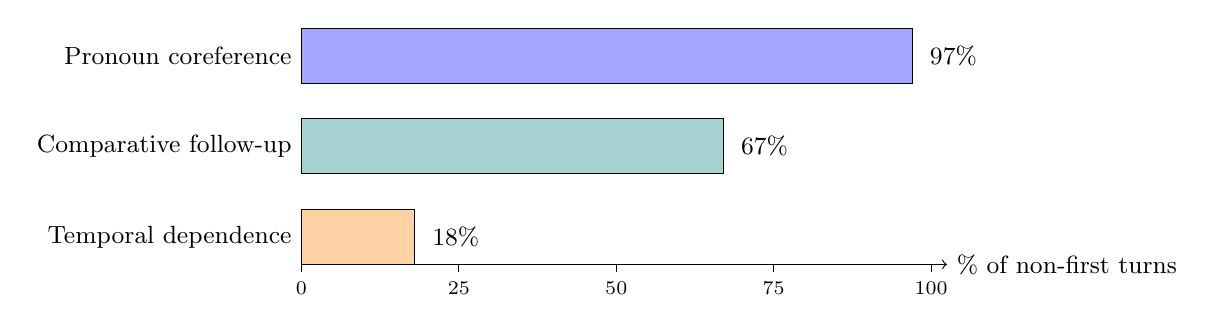
\begin{tikzpicture}
\begin{scope}
\draw[->] (0,0) -- (8.2,0) node[right, font=\small] {\% of non-first turns};
\foreach \x/\lbl in {0/0, 2/25, 4/50, 6/75, 8/100}
  \draw (\x,0) -- (\x,-0.1) node[below, font=\scriptsize] {\lbl};
\draw[fill=blue!35] (0,2.3) rectangle (7.76,3.0);
\node[left, font=\small] at (0,2.65) {Pronoun coreference};
\node[right, font=\small] at (7.86,2.65) {$97\%$};
\draw[fill=teal!35] (0,1.15) rectangle (5.36,1.85);
\node[left, font=\small] at (0,1.5) {Comparative follow-up};
\node[right, font=\small] at (5.46,1.5) {$67\%$};
\draw[fill=orange!35] (0,0) rectangle (1.44,0.7);
\node[left, font=\small] at (0,0.35) {Temporal dependence};
\node[right, font=\small] at (1.54,0.35) {$18\%$};
\end{scope}
\end{tikzpicture}
\caption{Distribution of non-standalone phenomena in the development set's non-first turns ($N{=}732$, multi-label: a single turn may exhibit more than one phenomenon simultaneously).}
\label{fig:nonstandalone-en}
\end{figure}

%==============================================================
\section{Key Architectural Challenges}
\label{sec:key-challenges}
%==============================================================

Based on the statistical properties of the corpus documented above, we identify three primary engineering bottlenecks that directly shape the system architecture of Chapter~5. We make explicit, for each challenge, which research question (Section~\ref{sec:rq}) it motivates.

\paragraph{1. Later-Turn Degradation (motivates RQ1).}
Unaugmented retrieval performance drops sharply after the first turn. Under ELSER v1 with raw, non-rewritten query formulations, Recall@5 falls from $0.879$ at Turn~1 to $0.428$ at Turns~$6{+}$, a $51\%$ relative drop, most of which occurs between Turns~1 and~2 (Section~\ref{sec:turn-depth}). This drop co-occurs with pronoun coreference (present in $97\%$ of non-first turns, Figure~\ref{fig:nonstandalone-en}) and comparative follow-ups ($67\%$), which systematically underspecify the query unless resolved against the history window---the empirical basis for RQ1's investigation of query diversity as a stabilization mechanism.

\paragraph{2. High Passage Diversity per Conversation (motivates RQ1).}
Conversations contain an average of $16.9$ unique relevant passages distributed across different source files. This high variance implies that the system cannot simply lock onto a single document block once found early in the conversation; it must dynamically adjust its search parameters at each turn to preserve breadth recall without flooding the generator's context with redundant or stale tokens.

\paragraph{3. The Test Set Distribution Shift (motivates RQ3).}
The held-out evaluation test set introduces severe distributional shifts relative to the development split, summarized in Table~\ref{tab:dev-test-en}. While the development split contains multi-turn threads averaging $7.7$ evaluated turns per conversation, every record in the test set consists of a \textit{single} evaluated turn embedded within a historical trace, and almost all of these turns ($465$ of $507$, $91.7\%$) are non-first turns that require contextual understanding, so the ``easy'' first-turn queries that inflate development-set averages are rare. Furthermore, the unanswerable rate nearly triples, from $6.5\%$ to $19.1\%$ globally, peaking in the Cloud domain at $27\%$ unanswerable turns. Systems whose answerability threshold is calibrated for the development set's low unanswerable rate therefore face precision degradation at test time due to this threshold mismatch---the central end-to-end finding developed in Section~\ref{sec:taskC-bottleneck}.

\begin{table}[h]
\centering
\small
\begin{tabular}{lcc}
\toprule
\textbf{Characteristic} & \textbf{Development} & \textbf{Test} \\
\midrule
Conversations & 110 & 507 \\
Total evaluated turns & 842 & 507 \\
Avg. turns/conversation & 7.7 & 1.0 \\
Answerable or partially answerable & $92.3\%$ & $74.4\%$ \\
\textbf{Unanswerable} & $6.5\%$ & $\mathbf{19.1\%}$ \\
Conversational / other & $1.2\%$ & $6.5\%^{\dagger}$ \\
\bottomrule
\end{tabular}
\caption{Development vs.\ test set comparison. The near-tripling of the unanswerable rate, combined with the predominance of non-first turns ($91.7\%$ of test turns), makes the test set substantially harder along both the retrieval and answerability-calibration axes. Development: $777$ answerable or partially answerable, $55$ unanswerable, and $10$ conversational turns. Test: $377$ turns with Task~A relevance judgments (answerable or partially answerable) and $97$ unanswerable turns. $^{\dagger}$The category of the remaining $33$ test turns could not be recovered from our records.}
\label{tab:dev-test-en}
\end{table}

%==============================================================
\section{Research Questions and Hypotheses}
\label{sec:rq}
%==============================================================

The thesis is organized around one central hypothesis:

\begin{quote}
\textit{The end-to-end performance of a multi-turn RAG system is limited primarily by the stability of retrieval across turns and by the calibration of the answerability gate, rather than by the expressive or synthesis capacity of current language models.}
\end{quote}

To examine it, this thesis investigates four Research Questions (RQs), each paired with a concrete, falsifiable hypothesis (H). The hypotheses address the retrieval and answerability parts of the central hypothesis; its final clause---that model capacity is not the binding constraint---is not tested directly, since we did not compare generators of different capability within Task~C.

\paragraph{RQ1:} Can structural query reformulation diversity substitute for heterogeneous retriever ensembling when targeting the vocabulary gap in deep dialogue turns?

\noindent \textbf{H1:} \textit{Fusing diverse, prompt-targeted query expansions over a single, highly corpus-aligned index captures complementary evidence pools without admitting the cross-domain ranking noise characteristic of multi-model retrieval ensembles.}

\paragraph{RQ2:} Does the introduction of a context bottleneck via verbatim evidence sentence extraction suppress parametric hallucinations without degrading the reference-based measures of answer quality?

\noindent \textbf{H2:} \textit{Restricting the generator's input to a compressed set of exact, extracted spans structurally bounds the token space available for hallucination, driving an asymmetric optimization in reference-less faithfulness metrics relative to reference-based metrics.}

\paragraph{RQ3:} How does the precision--recall trade-off of answerability gates behave under sudden, severe distribution shifts in unanswerable query density?

\noindent \textbf{H3:} \textit{Multi-layer answerability judges operating over independent signals (documents, spans, answers) reduce acceptance bias relative to a single-judge baseline, but nonetheless require distribution-adaptive threshold calibration to maximize harmonic-mean scores under high-unanswerable-rate test conditions.}

\paragraph{RQ4:} Can LLM-based reranking provide measurable gains over cross-encoder models when first-stage retrieval recall is close to saturation?

\noindent \textbf{H4:} \textit{Once first-stage retrieval recall approaches its Pareto upper bound ($R@100 > 0.90$), general-purpose LLM-as-a-judge listwise rerankers saturate, introducing substantial additional latency and cost for marginal or negative utility compared to optimized, specialized cross-encoders.}

These four hypotheses are evaluated empirically in Chapter~6: H1 and H4 are addressed jointly in the Task~A retrieval ablations (Section~\ref{sec:taskA-ablations}), H2 in the Task~B generation ablations (Section~\ref{sec:taskB-ablations}), and H3 in the Task~C answerability analysis (Section~\ref{sec:taskC-bottleneck}).

%==============================================================
\section{Formal Evaluation Methodology}
\label{sec:eval-methodology}
%==============================================================

System evaluation follows the strict tripartite protocol of MTRAGEval. Retrieval performance (Task~A) is quantified using Recall@$k$ (for $k \in \{5, 10, 50, 100\}$) and nDCG@5. Generation quality (Tasks~B and C) is measured via three complementary metrics, synthesized into a final Harmonic Mean (HM) leaderboard metric:

\begin{enumerate}
    \item \textbf{Reference-Based Algorithmic Score ($RB_{alg}$):} evaluates syntactic and sentence-level alignment against human-edited reference corrections, computed as an algorithmic fusion of BERT-Recall, BERT-K-Precision, and ROUGE-L.
    \item \textbf{Reference-Less Faithfulness Metric ($RL_F$):} derived from the RAGAS framework \citep{es2024ragas}, evaluating whether generated claims are strictly supported by the extracted evidence spans, independently of the human reference string.
    \item \textbf{Reference-Based LLM Judge ($RB_{llm}$):} a median-aggregated, multi-persona evaluator assessing three explicit criteria---Faithfulness (hallucination audit), Appropriateness (intent fulfillment and correct answerability handling), and Completeness (evidence coverage).
\end{enumerate}

The final leaderboard score is calculated as the harmonic mean of the three components:
\begin{equation}
\text{HM} = \frac{3}{\dfrac{1}{RB_{alg}} + \dfrac{1}{RL_F} + \dfrac{1}{RB_{llm}}}
\label{eq:hm}
\end{equation}

The choice of harmonic---rather than arithmetic---mean is deliberate and consequential: it strictly penalizes systems that exhibit asymmetric performance across the three axes (e.g., high fluency but low faithfulness due to hallucination), forcing balanced optimization across all three components rather than allowing strength on one axis to compensate for weakness on another. The additive objective of Equation~\eqref{eq:utility-decomposition} (Section~\ref{sec:unified-objective}) does not reproduce this property; it serves only as a conceptual decomposition of the task.

Crucially, an automated ``I Don't Know'' (IDK) classifier filters all response strings prior to scoring. Correct refusals on genuinely unanswerable turns are awarded a perfect score of $1.0$ across all three axes, whereas incorrect refusals on answerable turns, or false acceptances on unanswerable turns, receive a score of $0$. This scoring rule makes the answerability gate a high-stakes component of the end-to-end system alongside retrieval and generation quality, and motivates the answerability part of the central hypothesis stated in Section~\ref{sec:rq}.

%==============================================================
\section{Scope and Constraints}
\label{sec:scope}
%==============================================================

To situate the contributions of Chapter~5 correctly, we state explicitly what this thesis does and does not attempt, rather than leaving these boundaries implicit until the limitations discussion of Chapter~7.

\subsection{In Scope}

\begin{itemize}
    \item \textbf{All three MTRAGEval subtasks} (Sections~\ref{sec:formal-formulation}): passage retrieval (Task~A), reference-grounded generation (Task~B), and end-to-end RAG (Task~C), evaluated under the official competition protocol on both the development and held-out test splits.
    \item \textbf{Architectural and prompt-level interventions} over frozen, proprietary API models (DeepSeek-V3.2~\citep{deepseekai2024deepseekv3}, GPT-4o, GPT-4o-mini~\citep{openai2024gpt4o}): query reformulation strategy design, rank fusion algorithm design, evidence extraction and multi-candidate generation, and multi-judge answerability gating.
    \item \textbf{A single, corpus-aligned learned sparse retriever} (ELSER~v1) as the retrieval backbone, with retriever \emph{selection} itself treated as an empirical question addressed in Section~\ref{sec:taskA-ablations} rather than assumed a priori.
    \item \textbf{Development-set ablation of the main architectural components} introduced in Chapter~5 (query rewriting, retriever choice, reranking, the generation stages, the extractiveness band, and the answerability gate). Settings without a retained ablation---model routing, the per-corpus Nested RRF weights, the five-passage extraction limit, and the $60\%$ judge-invocation rate---are reported explicitly as design decisions (Sections~\ref{sec:model-routing} and~\ref{sec:additional-sweeps}).
\end{itemize}

\subsection{Out of Scope}

\begin{itemize}
    \item \textbf{Fine-tuning or parameter adaptation of any model.} No component of the pipeline---rewriter, generator, extractor, or judge---is fine-tuned on MTRAG data. Every reported gain is attributable to prompt engineering, architectural decomposition, and inference-time orchestration, not to gradient-based adaptation. Knowledge distillation into open-weight models is discussed only as future work (Section~\ref{sec:future-work}), not attempted here.
    \item \textbf{Cross-benchmark generalization.} The system is designed, tuned, and evaluated exclusively on MTRAG \citep{katsis2025mtrag}. We do not claim, nor do we evaluate, transfer to other conversational RAG benchmarks (e.g., TREC iKAT \citep{aliannejadi2024trec}, RAD-Bench \citep{kuo2025radbench}); the architectural principles of Chapter~5 are motivated by structural properties of multi-turn RAG that are plausibly shared across benchmarks, but this claim is not empirically tested in this thesis.
    \item \textbf{Distribution-adaptive calibration at inference time.} All thresholds and weights (the answerability confidence threshold $\tau$, the extractiveness band, the Nested RRF corpus weights) are tuned once on the development set and frozen for the test-set submission. As Section~\ref{sec:taskC-bottleneck} discusses, this static calibration is a likely major driver of the Task~C performance gap; online, distribution-adaptive calibration is scoped as future work rather than implemented here.
    \item \textbf{Non-English or cross-lingual retrieval and generation.} All four MTRAG corpora (Table~\ref{tab:corpus-stats-en}) are English-language; no claim is made about the system's behavior on multilingual or code-switched conversational input.
    \item \textbf{Human user studies and production deployment.} Evaluation is conducted exclusively against the offline MTRAGEval benchmark and its automated metrics (Section~\ref{sec:eval-methodology}); no live user study, latency-under-load measurement, or production A/B test is performed. Section~\ref{sec:limitations} discusses the orchestration engineering that would be required before such deployment.
\end{itemize}

This scope delineation follows directly from the unified optimization perspective of Section~\ref{sec:unified-objective}: the thesis addresses the architectural decomposition of $\mathcal{U}$ into retrieval, generation, and answerability sub-objectives, and the empirical validation of each sub-objective in isolation and in composition---not the orthogonal questions of model training, cross-domain transfer, or production-scale deployment engineering.
